\documentclass[a4paper, utf8]{ctexart}
\usepackage[fontset=Fandol]{ctex}
\usepackage{anyfontsize}
\usepackage{indentfirst}
\usepackage{enumitem}
\usepackage{fancyhdr}
\usepackage{geometry}
\usepackage{graphicx}
\usepackage{abstract}
\usepackage{amsmath}
\usepackage{lipsum}

% 设置页面间距
\geometry{a4paper,left=31mm,right=31mm,top=25mm,bottom=25mm}
% 章节标题左对齐
\CTEXsetup[format={\Large \bfseries}]{section}
% 段首缩进2字符
\setlength{\parindent}{2em}
% 设置页眉及页脚 页码
\pagestyle{fancy}
\fancyhf{}
\fancyhead[C]{}
\fancyhead[L]{HOMEWORK1:\ Exercises\ for\ Monte\ Carlo\ Methods}
\fancyhead[R]{21307210\ 傅祉珏}
\fancyfoot[C]{\thepage}
\fancyfoot[L,R]{}

% 使宋体可加粗
\setCJKfamilyfont{zhsong}[AutoFakeBold = {2.17}]{SimSun}
\renewcommand*{\songti}{\CJKfamily{zhsong}}

% 定义标题 作者及单位信息
\title{\songti \Large \textbf{HOMEWORK1:\ Exercises\ for\ Monte\ Carlo\ Methods}}
\author{Student\ ID:\ 21307210 \qquad Student\ Name:\ 傅祉珏}
\date{Lectured\ by\ 梁上松,\ Sun\ Yat-sen\ University}

\begin{document}
	
	\maketitle
	
	\section{Exercise\ 1}
	
	\subsection{Question}
	
	The Monte Carlo method can be used to generate an approximate value of $\pi$. The figure below shows a unit square with a quarter of a circle inscribed. The area of the square is 1 and the area of the quarter circle is $\pi/4$. Write a script to generate random points that are distributed uniformly in the unit square. The ratio between the number of points that fall inside the circle (red points) and the total number of points thrown (red and green points) gives an approximation to the value of $\pi/4$. This process is a Monte Carlo simulation approximating $\pi$. Let $N$ be the total number of points thrown. When $N=50, 100, 200, 300, 500, 1000, 5000$, what are the estimated $\pi$ values, respectively? For each $N$, repeat the throwing process 100 times, and report the mean and variance. Record the means and the corresponding variances in a table. 
	
	\begin{figure}[htbp]
		\centering
		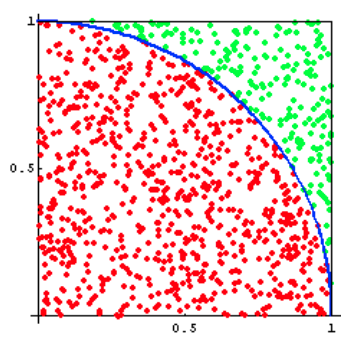
\includegraphics[width=.4\textwidth]{./figure/figure1.png}
		\caption{Using the Monte Carlo method to estimate $\pi$}
	\end{figure}
	
	\subsection{Answer}
	
	To use the Monte Carlo method to estimate the value of $\pi$, we first need to understand the basic geometric relationship. Inside a unit square, there is an inscribed quarter circle with a radius of 1. The area of the unit square is 1 square unit, while the area of the quarter circle is $\pi/4$ square units. By randomly generating points within the unit square and calculating the proportion of those points that fall inside the quarter circle, we can estimate the value of $\pi$.
	
	Specifically, we randomly generate $N$ points that are uniformly distributed within the unit square. For each point, we check whether its coordinates satisfy the equation of the circle $x^2 + y^2 \leq 1$. If it does, the point is inside the quarter circle; otherwise, it is outside. By calculating the ratio of the number of points that fall inside the circle to the total number of points $N$, we can obtain an approximate value for $\pi/4$. Since this ratio multiplied by 4 gives an approximation of $\pi$, we can use this ratio to estimate $\pi$.
	
	Following this concept, the code has been written, and the resulting code is shown in \verb|Exercises1.py|. Based on the requirements of the code, the following results can be obtained.
	
	\begin{table}[http]
		\begin{center}
			\caption{Exercises 1 Answer Table}
			\begin{tabular}{c c c c}
				\hline
				Index & N & Means & Variances \\
				\hline
				0 &   50 & 3.122400 & 0.054458 \\
				1 &  100 & 3.128800 & 0.025107 \\
				2 &  200 & 3.147600 & 0.015110 \\
				3 &  300 & 3.138133 & 0.010537 \\
				4 &  500 & 3.144560 & 0.005675 \\
				5 & 1000 & 3.141560 & 0.002618 \\
				6 & 5000 & 3.144552 & 0.000533 \\
				\hline
			\end{tabular}
		\end{center}
	\end{table}
	
	\section{Exercise\ 2}
	
	\subsection{Question}
	
	We are now trying to integrate the another function by Monte Carlo method:
	
	\begin{equation}
		\int_{0}^{1}x^3 dx
		\nonumber
	\end{equation}
	
	A simple analytic solution exists here: $\int_{0}^{1}x^3 dx=1/4$. If you compute this integration using Monte Carlo method, what distribution do you use to sample $x$? How good do you get when $N = 5, 10, 20, 30, 40, 50, 60, 70, 80, 100$, respectively? For each $N$, repeat the Monte Carlo process $100$ times, and report the mean and variance of the integrate in a table.
	
	\subsection{Answer}
	
	To integrate the function $ f(x) = x^3 $ over the interval $[0, 1]$ using the Monte Carlo method, we can follow these steps:
	
	\begin{enumerate}[itemsep=2pt, topsep=0pt, parsep=0pt]
		\item Sampling Distribution
	
		\item[] Since we are integrating over the interval $[0, 1]$, we will sample $x$ uniformly from this interval. This means we can use a uniform distribution $ U(0, 1) $.
	
		\item Monte Carlo Integration
	
		\item[] The Monte Carlo estimate for the integral is given by:
	
		\item[] \begin{equation} I \approx \frac{b-a}{N} \sum_{i=1}^{N} f(x_i) \nonumber \end{equation}
		
		\item[]	where $ [a, b] = [0, 1] $ and $ x_i $ are uniformly sampled points in the interval.
	
		\item Performing the Simulation
		
		\item[] We will repeat the Monte Carlo process for $ N = 5, 10, 20, 30, 40, 50, 60, 70, 80, 100 $ and perform 100 trials for each $N$.
	
		\item Calculating Mean and Variance
		
		\item[] For each $N$, we will calculate the mean and variance of the estimates from the 100 trials.
	\end{enumerate}
	
	Following this concept, the code has been written, and the resulting code is shown in \verb|Exercises2.py|. Based on the requirements of the code, the following results can be obtained.
	
	\begin{table}[http]
		\begin{center}
			\caption{Exercises 2 Answer Table}
			\begin{tabular}{c c c c}
				\hline
				Index & N & Means & Variances \\
				\hline
				0 &   5 & 0.245029 & 0.015738 \\
				1 &  10 & 0.259467 & 0.008685 \\
				2 &  20 & 0.257500 & 0.004301 \\
				3 &  30 & 0.248446 & 0.002323 \\
				4 &  40 & 0.246228 & 0.002289 \\
				5 &  50 & 0.252243 & 0.001301 \\ 
				6 &  60 & 0.250549 & 0.001021 \\
				7 &  70 & 0.246137 & 0.001154 \\
				8 &  80 & 0.248234 & 0.000905 \\
				9 & 100 & 0.247640 & 0.000868 \\
				\hline
			\end{tabular}
		\end{center}
	\end{table}
	
	\section{Exercise\ 3}
	
	\subsection{Question}
	
	We are now trying to integrate a more difficult function by Monte Carlo method that may not be analytically computed:
	
	\begin{equation}
		\int_{x=2}^{4} \int_{y=-1}^{1} f(x, y) = \dfrac{ y^2 \times e^{-y^2} + x^4 \times e^{-x^2}}{x \times e^{-x^2}}
		\nonumber
	\end{equation}
	
	Can you compute the above integration analytically? If you compute this integration using Monte Carlo method, what distribution do you use to sample $(x, y)$? How good do you get when the sample sizes are $N = 5, 10, 20, 30, 40, 50, 60, 70, 80, 100, 200$ respectively? For each $N$, repeat the Monte Carlo process 100 times, and report the mean and variance of the integrate.
	
	\subsection{Answer}
	
	First, we need to determine if the function can be integrated analytically over the specified limits. Given the complexity of $f(x,y)$, it's challenging to perform this integration directly. The integrand involves exponential terms and polynomial terms, making it unlikely that a simple closed form exists.
	
	The Monte Carlo method involves randomly sampling points from the region of integration and estimating the integral based on the average value of the function at those points. In this case, Since $x$ is constrained to the interval $[2,4]$ and $y$ to $[−1,1]$, we can use a uniform distribution to sample $x$ and $y$: For $x$, sample from $U(2,4)$; for $y$, sample from $U(−1,1)$.
	
	For each $N$, repeat the sampling process 100 times, generating $N$ samples of $(x,y)$ each time, and calculate the average value of $f(x,y)$ over these samples. Then estimate the integral by multiplying the average value by the area of the region, which is $4$. Finally, compute the mean and variance of the estimated integral values from the 100 repetitions.
	
	Following this concept, the code has been written, and the resulting code is shown in \verb|Exercises3.py|. Based on the requirements of the code, the following results can be obtained.
	
	\begin{table}[http]
		\begin{center}
			\caption{Exercises 3 Answer Table}
			\begin{tabular}{c c c c}
				\hline
				Index & N & Means & Variances \\
				\hline
				0 &    5 &  95200.743354 & 1.989497e+10 \\
				1 &  10 & 112027.570910 & 1.024562e+10 \\
				2 &  20 & 103470.545021 & 4.807861e+09 \\
				3 &  30 & 114248.092622 & 4.681874e+09 \\
				4 &  40 & 113754.545521 & 3.144835e+09 \\
				5 &  50 & 106303.688565 & 1.668617e+09 \\
				6 &  60 & 113812.281106 & 2.470408e+09 \\ 
				7 &  70 & 114186.319649 & 1.696168e+09 \\ 
				8 &  80 & 113507.130148 & 1.631517e+09 \\ 
				9 & 100 & 115568.852197 & 1.197880e+09 \\ 
				10 & 200 & 113505.642425 & 7.224751e+08 \\
				\hline
			\end{tabular}
		\end{center}
	\end{table}
	
	\section{Exercise\ 4}
	
	\subsection{Question}
	
	An ant is trying to get from point $A$ to point $B$ in a grid. The coordinates of point $A$ is \  $(1,1)$ (this is top left corner), and the coordinates of point $B$ is $(n,n)$ (this is bottom right corner, $n$ is the size of the grid).
	
	Once the ant starts moving, there are four options, it can go left, right, up or down (no diagonal movement allowed). If any of these four options satisfy the following:
	
	(a) The new point should still be within the boundaries of the $n\times n$ grid
	
	(b) Only the center point $(4, 4)$ is allowed to be visited zero, one or two times, while the remainder points should not be visited previously (are allowed to be visited zero or one time).
	
	If $P$ is the probability of the ant reaching point $B$ for a $7\times7$ grid, use Monte Carlo simulation to compute $P$. Pick the answer closest to $P$ in value (assume $20,000$ simulations are sufficient enough to compute $P$).
	
	\begin{figure}[htbp]
		\centering
		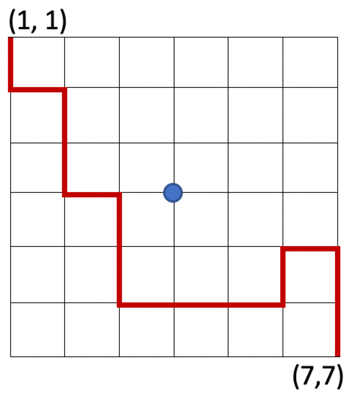
\includegraphics[width=.4\textwidth]{./figure/figure2.png}
		\caption{An ant is trying to get from point $A(1,1)$ to point $B(7,7)$ in a grid}
	\end{figure}
	
	\subsection{Answer}
	
	To estimate the probability $P$ of the ant reaching point $B$ in a $7 \times 7$ grid using Monte Carlo simulation, we first set the grid range from $(1, 1)$ to $(7, 7)$, where the center point $(4, 4)$ can be visited up to two times, while other points can only be visited once. The ant can move in four directions: left, right, up, or down, while ensuring that movements remain within the grid boundaries. The simulation continues until the ant reaches $(7, 7)$ or can no longer move without violating the visiting rules. We will conduct a total of $20,000$ simulations and count the number of successful trials, i.e., the times the ant reaches $(7, 7)$. Finally, we calculate $P$ as the ratio of successful trials to the total number of trials.
	
	Following this concept, the code has been written, and the resulting code is shown in \verb|Exercises4.py|. Based on the requirements of the code, the probability of the ant reaching point $B$ for a $7 \times 7$ grid is $25.5\% \pm 0.5\%$.
	
	\section{Exercises\ 5}
	
	\subsection{Question}
	
	Given a system made of discrete components with known reliability, what is the reliability of the overall system? For example, suppose we have a system that can be described with the following high-level diagram in 图3.
	
	\begin{figure}[htbp]
		\centering
		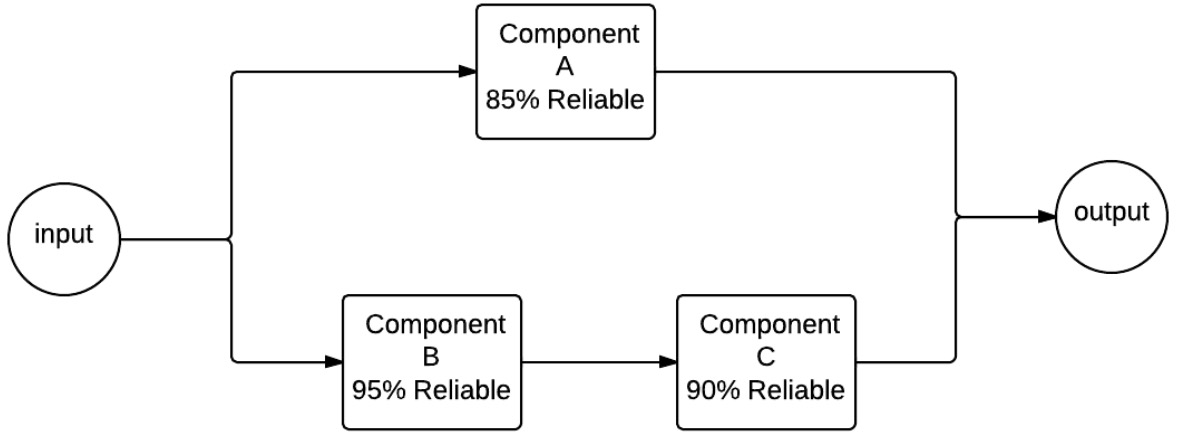
\includegraphics[width=.75\textwidth]{./figure/figure3.png}
		\caption{A system made of discrete components}
	\end{figure}
	
	When given an input to the system, that input flows through component $A$ or through components $B$ and $C$, each of which has a certain reliability of correctness. Probability theory tells us the following:
	
	\begin{equation}
		\begin{aligned}
			reliability_{BC}&=0.95\times0.90=0.855 \\
			reliability_A&=0.85
		\end{aligned}
		\nonumber
	\end{equation}
	
	And the overall reliability of the system is:
	
	\begin{equation}
		\begin{aligned}
			reliability_{sys}&=1.0-[(1.0-0.85)\times(1.0-0.855)] \\
			&=0.97825
		\end{aligned}
		\nonumber
	\end{equation}
	
	Create a simulation of this system where half the time the input travels through component $A$. To simulate its reliability, generate a number between $0$ and $1$. If the number is $0.85$ or below, component A succeeded, and the system works. The other half of the time, the input would travel on the lower half of the diagram. To simulate this, you will generate two numbers between $0$ and $1$. If the number for component $B$ is less than $0.95$ and the number for component $C$ is less than $0.90$, then the system also succeeds. Run many trials to see if you converge on the same reliability as predicted by probability theory.
	
	\subsection{Answer}
	
	Based on the research question's requirements, this study uses conditional statements to filter randomly generated number sequences by applying specified conditions. The success count is then divided by the total number of attempts to calculate the final probability value. Following this concept, the code has been written, and the resulting code is shown in \verb|Exercises5.py|. However, in the experiment, if half of the data passes the first stage and the other half passes the second stage, the probability obtained through programming is \(85.25\% \pm 0.25\%\), which significantly differs from the theoretical calculated value of \(0.97825\%\). Through mathematical expression and analysis, this study identifies that the original calculation method incorrectly considered the probability of data failing both $A$ and $B$ and $C$, rather than the success probability of data passing $A$ or $B$ and $C$. Consequently, the code was revised to classify any data passing $A$ or $B$ and $C$ as a success. After this correction, the probability calculation result was \(97.80\% \pm 0.10\%\), which statistically aligns with the theoretical calculated value.
	
\end{document}